\section*{Test problems}

\subsection*{Branin (heteroscedastic, 5 levels)}
$$f(x_1,\ell)=\Big(x_2(\ell)-\tfrac{5.1}{4\pi^2}x_1^2+\tfrac{5}{\pi}x_1-6\Big)^2
+10\Big(1-\tfrac{1}{8\pi}\Big)\cos x_1+10,\quad x_1\in[-5,10],\ x_2(\ell)\in\{15,2,8,0,10\}$$
$$\sigma(x_1,\ell)=\Big[0.5+0.15(x_1+5)+\tfrac{2.5}{1+e^{-1.2(x_1-2)}}\Big]\,m(\ell),
\quad m(\ell)\in\{0.5,1.0,1.8,2.5,3.5\}$$
\begin{center}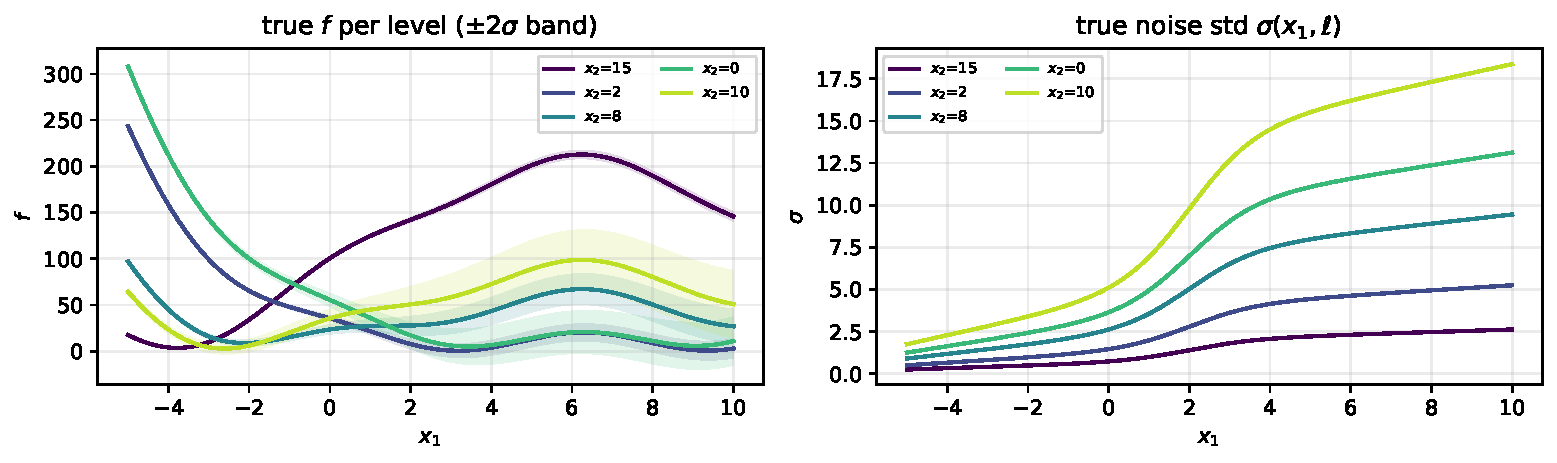
\includegraphics[width=0.85\linewidth]{figs/branin_truth.pdf}\end{center}

\subsection*{Six-hump camel (5 levels: two pairs + bridge)}
$$f(x_1,\ell)=\Big(4-2.1x_1^2+\tfrac{x_1^4}{3}\Big)x_1^2+x_1 x_2(\ell)+(-4+4x_2(\ell)^2)x_2(\ell)^2,
\quad x_1\in[-2,2],\ x_2(\ell)\in\{-1.0,-0.85,0.0,0.85,1.0\}$$
$$\sigma(x_1,\ell)=0.05\,e^{(0.4x_1)^2}\,m(\ell),\quad m(\ell)\in\{2.0,3.5,1.5,5.0,2.5\}$$
(noise as used in the 30-seed replication tables below)
\begin{center}
\includegraphics[width=0.85\linewidth]{figs/camel_truth_v40.pdf}\end{center}

\subsection*{Friedman 5-D + categorical (shape-only level pairs)}
$$f_\ell(\mathbf{x})=a(\ell)\cdot 10\sin(\pi x_1 x_2)+20(x_3-0.5)^2+b(\ell)\cdot 10x_4+5x_5,
\quad \mathbf{x}\in[0,1]^5$$
$$a(\ell)\in\{1.0,0.85,0.5,0.35\},\quad b(\ell)\in\{1.0,1.1,1.5,1.65\},\quad
\sigma(\mathbf{x},\ell)=0.1\cdot 10^{\,x_1-0.5}\;m(\ell),\quad
m(\ell)\in\{1.5,1.0,3.0,2.0\}$$
\begin{center}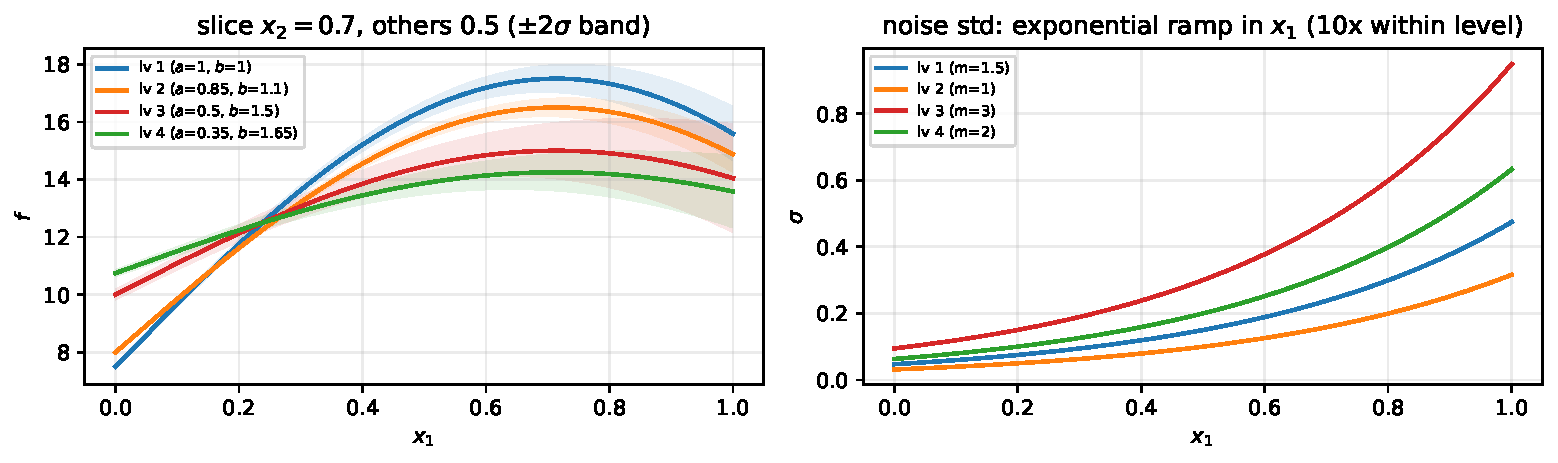
\includegraphics[width=0.85\linewidth]{figs/friedman_truth.pdf}\end{center}
\clearpage
